%%%%%%%%%%%%%%%%%%%%%%%%%%%%%%%%%%%%%%%%%%%%%%%%%%%%%%%%%%%%%%%%%%%%
%-------------------------------------------------------------------
% Agile Software Development Methods
%-------------------------------------------------------------------
%%%%%%%%%%%%%%%%%%%%%%%%%%%%%%%%%%%%%%%%%%%%%%%%%%%%%%%%%%%%%%%%%%%%
\selectlanguage{british}
\chapter{Agile Software Development Methods}
\label{toc:agile}

Software developers are beginning to realise that traditional, 
waterfall-style development methods are starting to fall apart in the 
rapidly changing business software development field 
\citep{betterway}. The waterfall model, which consists of all the 
standard software development phases lined up one after the other 
\citep{softwareeng}, is the oldest software life-cycle model and has 
been widely used in both large and small projects \citep{agilequality} 
with successes especially in large and complex projects. However, at 
the very core of the waterfall model is the idea of planning 
everything at the beginning of the project. Change is not an aspect 
that is anticipated in waterfall-based development, and change is what 
the modern business software development is all about. Trying to 
decide everything as early as possible means being unable to adapt to 
new business conditions, which leads to business failure 
\citep{agileinnovation}. In the present situation, the waterfall model 
just does not work \citep{betterway}. There is a demand for new models 
that allow developers to change the plans even later on.

In this chapter, the relatively new agile approach to software 
development is presented. First, an overview of the agile processes is 
given. Then, the two major agile processes, Extreme Programming and 
Scrum are introduced in consecutive sections. Finally, an approach for 
adopting agile methods is proposed.


%%%%%%%%%%%%%%%%%%%%%%%%%%%%%%%%%%%%%%%%%%%%%%%%%%%%%%%%%%%%%%%%%%%%
% Overview
%%%%%%%%%%%%%%%%%%%%%%%%%%%%%%%%%%%%%%%%%%%%%%%%%%%%%%%%%%%%%%%%%%%%
\section{Overview}
\label{toc:agile:overview}

The need for models that embrace change has been identified. Most of 
the traditional waterfall-based software development projects, which 
have been planned as far as possible, still have to change. 
\cite{agileinnovation} report that in a study of more than 200 
software projects, nearly half of them did not have their original 
plans in use at the end of the project. Conforming to the plans had 
not been the primary goal anymore, and the projects had to respond to 
requirement changes instead.

Agile development methods promise to bring a solution to this need. 
They take a different perspective to software development in 
comparison to the waterfall model. The basic lesson in software 
engineering has been that the cost of change increases exponentially 
as the software moves towards production use \citep{softwareeng}. The 
motivation has been to identify and carry out changes as early as 
possible. However, with a proper combination of technology and 
programming practices, it is possible to stop the cost of change from 
increasing \citep{xpexplained}. In agile software development, 
responding to change is emphasised.

Accepting change and allowing large-scale changes later on in a 
project is not enough, however. If the cost of changes still rises 
exponentially as the project proceeds towards production, changing 
requirements at a later phase can still lead the project to a disaster 
\citep{xpexplained}. The possible solutions must supply a way to stop 
the increase of the cost of change, or at least to slow it down. In 
the waterfall model, the cost comes from having to redo the entire 
development cycle. To carry out a requirement change to a software 
that is in its maintenance phase, a developer must change the 
requirements, redo the specifications and design, implement the change 
and retest the entire application to ensure that everything is still 
working \citep{softwareeng}. The cost, therefore, comes from having to 
maintain a multitude of documents and having to carry out extensive 
and expensive tests. Implementing the change might not be easy either, 
if the architecture has not been developed with changeability in mind. 
Agile methods respond to these requirements by requiring less 
documentation, making the software easier to change and by having 
automated unit tests to support software changes.


% Documentation
% -------------
\subsection{Documentation}
\label{toc:agile:overview:documentation}

For documentation, the agile viewpoint is that there should only be 
the bare minimum of it. \cite{agilesd} sees software development as a 
game that has the production of the actual software as its primary 
goal. Maintaining extensive documentation is a primary requirement 
only for setting up the next game, as the updated documentation is 
only needed to make it possible for new developers to understand the 
system. In the gamer's perspective, setting up the next game is only a 
secondary goal. If the primary goal is not reached, the game ends in 
any case. Therefore, there should only a \textsl{sufficient} amount of 
documentation.


% Testing
% -------
\subsection{Testing}
\label{toc:agile:overview:testing}

Testing is another important aspect of agile methods. In contrast to 
the waterfall model, which places testing at the end of the 
development cycle, most agile methods advocate test-driven development 
(\abbrev{TDD}), which states that tests must be written before the 
code itself \citep{xpexplained} and that a failing test must be 
written before a defect is fixed \citep{questioningxp}. In addition, 
every program feature must be covered with tests. These tests are 
written as automated unit tests, which should always run at 100\% 
success, except during the time when implementing a new feature or 
fixing a defect \citep{xpexplained}. These tests provide rapid 
feedback on the effects of a change.

The \abbrev{XP} method (see section~\ref{toc:agile:xp}) suggests that 
unit tests and functional acceptance tests are sufficient for a 
project \citep{xpexplained}. While these tests are not necessarily as 
good as tests created by professional testers, organisations adopting 
\abbrev{XP} have discovered that the quality of the software itself is 
better \citep{questioningxp}. Test-driven development is one of the 
essential \abbrev{XP} practices, which should always be included even 
when adopting the practice incrementally \citep{xpapplied}. 
\cite{agileadoption} reports an immediate decrease of defect counts, 
from 20--30 to only a few per iteration, with the adoption of 
test-driven development.


% Simple Design
% -------------
\subsection{Simple Design}
\label{toc:agile:overview:design}

To keep the code easy to change, agile methods favour a simple design. 
The idea is to develop the simplest solution that could possibly work 
for the current feature \citep{xpexplained}. Since the future is 
uncertain, it is useless to try to design the system as it is at the 
end of the project. If and when the design solution is not good enough 
anymore, it is \textsl{refactored}\footnote{Refactoring means changing 
the current internal structure of the code without changing its 
external behaviour \citep{xpapplied}.} to meet the new requirements. 
Refactoring must also be used to keep the software structure as simple 
as it can be and to remove duplicated code. This idea of 
\textsl{designing through refactoring} keeps the code clear and allows 
developers to design only what is required to implement the next 
feature. \citep{xpexplained}

Without the extensive unit test cases that need to be built, the 
developers might be unwilling to perform the required refactorings to 
keep the code simple. However, the unit tests provide the safety nets 
that are required to assure the developer that everything is still 
working after the change is done. \citep{questioningxp}


% Softwate quality
% ----------------
\subsection{Software Quality}
\label{toc:agile:overview:quality}

Because the design is simple, not planned totally up front, and the 
documentation is light, the quality of the produced code can be seen 
as questionable by traditional waterfall model proponents 
\citep{agilequality}. However, the agile methods do have quality
attributes.

First of all, as noted before, test-driven development has been seen 
to reduce the amount of simple defects \citep{agileadoption} and 
simple design that is frequently refactored reduces unnecessary code 
complexity and maintains higher code quality \citep{betterway}. Agile 
methods also include \textsl{continuous integration} (see 
section~\ref{toc:agile:xp}), which means that code is integrated to 
the code base as soon as it is ready \citep{agilesdm}. This reduces 
the defects introduced with massive infrequent integrations. In 
addition, the acceptance tests can also be automated 
\citep{xpapplied}. In theory, all the tests a software system needs 
could be run with a single command. In conclusion, with agile methods 
the quality checking practices happen with a higher frequency than in 
the waterfall development method, and they are available earlier 
\citep{agilequality}.


% The Agile Alliance
% ------------------
\subsection{The Agile Alliance}
\label{toc:agile:overview:agilealliance}

In early 2001, seventeen advocates of lightweight development 
processes gathered together in Utah and formed a group called the 
Agile Alliance \citep{agilealliance,agilesd}. In their meeting they 
produced the Agile Manifesto \citep{manifesto}, which lays down the 
basics for agile development methods. The manifesto presents the 
viewpoint that agile development should have. The values of agile 
manifesto are listed below. The manifesto acknowledges the values of 
the items on the right side, but holds the items on the left side more 
important.

\begin{description}
  \item[Individuals and interactions] over processes and tools
  \item[Working software] over comprehensive documentation
  \item[Customer collaboration] over contract negotiation
  \item[Responding to change] over following a plan
\end{description}

The values emphasise the human role as opposed to industrial 
processes. A working team spirit is important in the agile methods. 
The second point underlines the importance to continuously produce 
new, working versions of the software, with short release periods. The 
third point sets great store by creating good relationships with the 
customer instead of negotiating strict contracts. Finally, the ability 
to make changes to the software even later on in the project is 
highlighted. \citep{agilesdm}


%%%%%%%%%%%%%%%%%%%%%%%%%%%%%%%%%%%%%%%%%%%%%%%%%%%%%%%%%%%%%%%%%%%%
% Extreme Programming
%%%%%%%%%%%%%%%%%%%%%%%%%%%%%%%%%%%%%%%%%%%%%%%%%%%%%%%%%%%%%%%%%%%%
\section{Extreme Programming}
\label{toc:agile:xp}

The development of \abbrev{XP} started from the problems noticed with 
the long development cycles in the traditional software development 
models. The first motivation was to create a method for simply getting 
the work done, and the theoretical basis was established after a 
number of successful trials in practice \citep{agilesdm}. \abbrev{XP} 
is a lightweight method that is designed for small-to-medium sized 
teams developing software with rapidly changing requirements 
\citep{xpexplained}. \abbrev{XP} has been the most popular agile 
methodology \citep{rapidxp}, and has been widely accepted as the most 
important one \citep{agilescrum}.

\abbrev{XP} has been very successful in its area of applicability 
\citep{agilesd}, and mostly successful experiences have been reported 
when using it \citep{agilesdm}. Programmers like to develop with 
\abbrev{XP}, since in \abbrev{XP} they get to do more actual 
programming work \citep{xpexplained}. However, \cite{questioningxp} 
sees a big problem in this. Since developing with \abbrev{XP} is more 
fun than doing things the traditional way, developers inflected with 
\abbrev{XP} might not want to change back to using the traditional 
methods when their usage is required, for example with large and 
complicated projects that have well-known requirements.


% Practices
% ---------
\subsection{Practices}
\label{toc:agile:xp:practices}

At the core of \abbrev{XP} are twelve simple practices, which are 
listed in this chapter. None of these practices are new in software 
engineering \citep{xpexplained}. The promise of \abbrev{XP} is to 
bring them together in a way that produces the most benefits. The 
\textsl{extreme} in Extreme Programming comes from taking these 
standard practices to extreme levels \citep{agilesdm}. The practices 
listed here have been taken from 
\citep{xpapplied,xpexplained,agilesd,rapidxp}.

\begin{description}
\item[Planning Game] The planning game in \abbrev{XP} is \abbrev{XP}'s 
response to the problem that you cannot know everything beforehand, 
especially in software engineering. The main idea in planning game is 
to form a rough plan of the next iteration quickly, and then refine it 
as the iteration moves on. The planning game is a collaborative game 
with the customer and the developers working closely together. The 
developers participate by estimating how much implementing a software 
feature will cost, and the business people must decide which features 
will be included to the iteration and what are their priorities.

\item[Short Releases] \abbrev{XP} emphasises that new versions of the 
software should be released often, in iterations of one or two months, 
rather than once or twice a year. Frequent iterations provide early 
value to the customer. In addition, the customer is quickly able to 
verify that the developed software is working as required, thus 
reducing customer risk and providing valuable feedback to the 
development team. The iterations must still produce complete features.

\item[Metaphor] A metaphor in \abbrev{XP} is a shared story between 
the customer and the developers. It creates a common vocabulary and 
guides the developers when designing the software. The \abbrev{XP} 
metaphor replaces the architecture in traditional software. An example 
of a metaphor is, for example, an assembly line, which could be used 
to describe customer help desk. Phone calls could be seen as items 
that are passed through different persons (working at the assembly 
line). This provides a way to look at the software at a familiar 
angle, and helps raise questions such as "what happens when the item 
(phone call) reaches the end of the line?"

\cite{agileadoption} reports of a project that was having problems 
with certain interface code that did not have any consistent 
structure. They identified the lack of any guiding metaphor as the 
problem. As a solution, a metaphor was sought and found, and the 
existing messed-up interface code was refactored a bit at a time to 
match the new metaphor. After a few iterations the interface code had 
been cleaned and implementing new features was easier.

\item[Simple Design] Generally software design is "implemented for 
today and planned for tomorrow" \citep{xpexplained}. \abbrev{XP} 
states that since you cannot know the future, you should not try to 
make extensive plans for it. The design of a software must always be 
as simple as possible. This means that the software must run all 
tests, have no duplicate logic, state every intention that is 
important and have the fewest possible classes and methods. The 
software must not contain any functionality that is not currently 
needed, because the need for that functionality might never arise.

\item[Testing] \abbrev{XP} contains two types of testing, namely, unit 
testing and functional acceptance testing. \abbrev{XP} applies 
test-driven development with the developers writing the unit tests, 
and the customer provides the functional tests. All unit tests must 
pass at all times (except during the actual development of a new 
feature or when fixing a defect). Functional tests, on the other hand, 
can fail, as they are used to measure the development progress. When 
all functional tests complete successfully, the software is ready. 
Testing is one of the few necessary aspects of \abbrev{XP}, even when 
adopting the method incrementally. If you do not write tests, you are 
not being extreme \citep{xpexplained}.

\cite{tddvswaterfall} report that projects using \abbrev{TDD} have 
produced software that is more reliable, easier to maintain and more 
efficient, and have produced it up to 10\% faster than with 
traditional methods.

\item[Refactoring] Refactoring is the process of changing the internal 
structure of the code without changing its functionality. Refactoring 
is applied to remove duplication, to improve communication, to 
simplify the design and to add flexibility. When adding a new feature, 
developers look at the code and think of ways of changing it so that 
adding the feature is easier. After adding the feature, developers can 
look at the code and think of ways to simplify the resulting design. 
These are both forms of refactoring. Because refactoring often 
requires changes to many parts of the system, extensive unit tests are 
needed to assure the developer that everything is still working 
afterwards. While a single structural change is usually quite small, 
multiple consecutive refactoring changes can be used to achieve large 
restructurings with less chances of breaking the application code 
\citep{agilequality}.

\item[Pair Programming] In pure \abbrev{XP}, every line of code is 
written in pairs, with two developers working on one computer. The one 
holding the keyboard and mouse is reflecting on the best way to 
implement the actual method under work, and the other one is looking 
at the general view, thinking of the consequences and possible 
simplifications. The pairs switch their roles every now and then. 
Although the method may seem inefficient, it provides several 
important benefits. Every part of the system is familiar to at least 
two developers, and when working as a pair, the developers motivate 
each other to better development practices. The developers pair with 
different people frequently, thus spreading the knowledge of the 
system inside the team.

Most experiences with pair programming have been positive. 
\cite{strengtheningpair} report that developers who have used pair 
programming have worked harder and smarter, and have produced results 
early. \cite{agileadoption} describes that a team considered pair 
programming too wasteful of resources at first, but later on developed 
the motivation for using it. In that team pair programming had helped 
spread out expert knowledge from a single developer and had thus 
removed a bottleneck.

\item[Collective Ownership] Collective ownership means that each 
developer is allowed to change any part of the code at any time. 
Having the right to change code is a basic requirement to be able to 
apply refactoring. Without control, this could lead to chaos. This is 
mitigated in \abbrev{XP} by making everyone responsible for the entire 
code, and by having the unit tests that should run at all times. If 
developers break something, they must fix it so that the unit tests 
run again.

\item[Continuous Integration] Code is integrated to the version 
control system frequently, at least once every day. Each pair 
integrates their modifications, and after the integration, all unit 
tests should run. This removes the integration nightmare that happens 
when integration is left at the end of a development phase, and 
possible integration problems arise earlier on in the project.

\item[40-hour Week] Developers must not work more than 40 hours a 
week. Overtime is accepted for one week, but never for two consecutive 
weeks. Having to work overtime is an indication of a problem for which 
working overtime is not the solution. Developers cannot produce the 
required quality when working overtime.

\item[On-Site Customer] A real customer representative should be 
physically present at the development site full-time. The customer can 
do other work at the time, but he must be available for the team to 
clarify user stories\footnote{User stories are \abbrev{XP}'s 
counterpart for requirements.} and make business decisions.

\item[Coding Standards] Since all software code is being modified by 
everyone, the team must adopt a single coding practice that is 
accepted and followed by all team members. Developers should not be 
able to recognise who wrote which piece of code. Without an accepted 
standard development time will be lost on code style questions.
\end{description}


% Common Problems
% ---------------
\subsection{Common Problems}
\label{toc:agile:xp:problems}

There are several problems identified when using \abbrev{XP}. As noted
before, \cite{questioningxp} surmises that developers who have used
\abbrev{XP} might not be willing to switch back to traditional,
waterfall-type software methods. Another point is the scalability of
the process. According to \cite{rapidxp}, there is no real data
available on how well \abbrev{XP} scales for larger teams.
\cite{xpexplained} suggests using around ten developers in an
\abbrev{XP} team.


%%%%%%%%%%%%%%%%%%%%%%%%%%%%%%%%%%%%%%%%%%%%%%%%%%%%%%%%%%%%%%%%%%%%
% Scrum
%%%%%%%%%%%%%%%%%%%%%%%%%%%%%%%%%%%%%%%%%%%%%%%%%%%%%%%%%%%%%%%%%%%%
\section{Scrum}
\label{toc:agile:scrum}

Scrum is an agile, lightweight and adaptable process for managing 
systems development with small teams. Scrum does not define any 
specific development methods for the implementation phase, but 
concentrates on how the team members should function in order to 
produce the required system in a constantly changing business 
environment. \citep{scrum,agilesdm}

Scrum starts with the assumption that software development involves 
several variables that are likely to change during the project. These 
include requirements, resources, time frame and technology 
\citep{agilesdm}. Instead of trying to plan these in detail in 
advance, Scrum defines an empirical process control for ensuring that 
the current status of the project is visible, inspected and the 
methods are adapted to function in new situations 
\citep{agilescrum}.

At the core of Scrum is an iterative, incremental process skeleton, 
which is shown in figure~\ref{fig:scrumskeleton}. Scrum is an 
iterative process: a project using Scrum is divided into 
\textsl{sprints}, which are the iterations of Scrum. Scrum is also 
incremental: each sprint produces a working, shippable version of the 
software with additional functionality.

\begin{figure}
\begin{center}
  \epsfig{file=images/scrumskeleton.eps, width=90mm}
  \caption{The Scrum Skeleton (adapted from \citep{agilescrum})}
  \label{fig:scrumskeleton}
\end{center}
\end{figure}

The actual Scrum process is built on top of the skeleton. The process 
contains three phases: \textsl{pregame}, \textsl{development} and 
\textsl{post-game}. Before the project begins, the project teams, 
tools and other resources are defined in the pregame phase. The 
pregame phase also contains the high-level architecture definition of 
the system. The development phase is the agile part of Scrum, in which 
the software is implemented in sprints. All variables that can change 
(such as requirements and resources) are observed and controlled 
through various Scrum practices. After there are no more requirements 
for the software, the project moves to the post-game phase, in which 
the finalised software is documented and released. \citep{agilesdm}


% Roles
% -----
\subsection{Roles}
\label{toc:agile:scrum:roles}

To implement the iterative, incremental skeleton shown in 
figure~\ref{fig:scrumskeleton}, Scrum defines three roles for project 
members \citep{apmscrum,agilescrum}. These roles are described below.

\begin{description}

\item[Product Owner] The product owner represents the business
viewpoint of the project by providing the initial overall requirements,
objectives and release plans. The product owner is also responsible for
prioritising the requirements throughout the project.

\item[Team] The team is responsible for developing the functionality 
in the sprints. The team is a self-organising unit who is solely 
responsible for producing the required functionality at the end of the 
iteration. The team itself selects the development methods used in the 
project and assigns the development tasks. A good size for a Scrum 
team is not more than ten people. The motivation for this is that 
small teams that work independently are more effective 
\citep{scrumprocess}.

\item[ScrumMaster] The ScrumMaster is Scrum's counterpart for a 
project manager. In contrast to a traditional project manager, a 
ScrumMaster does not lead the team, but rather acts as a coach. The 
ScrumMaster is responsible for maintaining the Scrum process and for 
teaching Scrum to everyone included.

\end{description}

A crude summary of the role distribution is that the product owner 
gives and prioritises the requirements, and all project members decide 
what should be developed in the next sprint. The team is then left 
alone to produce the required functionality, with the ScrumMaster 
supervising the correct usage of Scrum methods and acting as a mentor. 
In addition to these, \cite{agilesdm} identify the roles of 
\textsl{customer}, \textsl{management} and \textsl{user}. These roles 
are largely related to setting the goals and requirements.

Perhaps most importantly, Scrum divides the project stakeholders into 
those who are \textsl{committed} and those who are only 
\textsl{involved}. The product owner, the Scrum team and the 
ScrumMaster are all committed to the project, but another manager 
interested in the project would only be involved. In Scrum, only the 
committed people have a right to decide about project issues.

\cite{apmscrum} reports of projects that had not worked as well as 
they could have when people had not filled the roles properly. For 
example, if the ScrumMaster tries to lead the team in the same way as 
a traditional project manager, the team does not achieve the 
commitment and productivity that can emerge when they are left to find 
out the best methods by themselves.


% Practices
% ---------
\subsection{Practices}
\label{toc:agile:scrum:practices}

To control the chaos caused by unpredictability and complexity, Scrum 
defines a set of practices, which are listed below. The practices have 
been taken from \citep{agilesdm,apmscrum,scrumprocess}.

\begin{description}

\item[Product Backlog] The product backlog of Scrum contains the 
prioritised requirements of the software to be developed. The product 
backlog is never completed during the project, but it is always 
updated when new requirements are discovered or current ones are 
refined. When all items in the backlog have been finished, the project 
is complete. The product owner is responsible for maintaining the 
product backlog.

A tool for maintaining the product backlog item status is the 
\textsl{burndown chart}, which is a table that can be used for 
tracking the items. It shows the amount of work remaining for each 
item across iterations.

\item[Effort Estimation] Effort estimation in Scrum is an iterative 
process. At first, initial estimates are filled to the product backlog 
(or burndown chart). After more accurate estimations are formed, the
new estimates are added as new columns to the burndown chart. This way
the whole estimate history can be tracked from the burndown chart.

\item[Sprint] At the heart of Scrum are the sprints. A sprint is 
originally a 30-day iteration, but \cite{scrumprocess} relax the 
length requirement into one to four weeks. Each sprint delivers 
valuable functionality to the developed system. During a sprint, the 
Scrum team selects the appropriate methods for reaching that goal, 
with the aid of the ScrumMaster.

\item[Sprint Planning Meeting] Before each sprint a two-part sprint 
planning meeting is held. In the first part of this meeting the goals 
for the next sprint are decided and prioritised. The product owner 
selects the most important features from the product backlog, and the 
team then tells how many of these they can implement during the 
sprint. In the second part, the team lays down preliminary plans for 
the sprint by creating tasks to the \textsl{spring backlog}.

\item[Sprint Backlog] The sprint backlog is the starting point for 
each sprint. Initially, a set of requirements is taken from the 
product backlog and expanded into the sprint backlog. These are then 
refined during the sprint, but new requirements are not added to the 
list. New requirements can only be added to the product backlog.

\item[Daily Scrum Meeting] To keep every project member up-to-date 
with the current situation, Scrum introduces daily Scrum meetings. 
These meetings are short status meetings that follow a very 
well-defined form. In each meeting, every developer is asked three 
questions: \textsl{what has the developer done since the last 
meeting}, \textsl{what does the developer plan to do before the next 
meeting}, and \textsl{are there any obstacles in the developer's way}. 
The purpose of these formal questions is to keep the meeting focused 
but still allow everyone to get a clear picture of how the project is 
proceeding. Any problems identified are not discussed in the meeting, 
but another meeting will be scheduled for the team members who should 
discuss the problem.

\cite{scrumprocess} report that developers enjoy the small successes 
that arise from being able to say that they have finished their tasks. 
The meetings have also been useful as other developers have often 
battled with the same problems and could share their experiences after 
the daily meeting.

\item[Sprint Review Meeting] After each iteration, a sprint review 
meeting is held. In this meeting the produced software is introduced 
to the rest of the project stakeholders. In the meeting the contents 
of the next sprint are also discussed.
\end{description}



%%%%%%%%%%%%%%%%%%%%%%%%%%%%%%%%%%%%%%%%%%%%%%%%%%%%%%%%%%%%%%%%%%%%
% Adopting an Agile Process
%%%%%%%%%%%%%%%%%%%%%%%%%%%%%%%%%%%%%%%%%%%%%%%%%%%%%%%%%%%%%%%%%%%%
\section{Adopting an Agile Process}
\label{toc:agile:adopt}

When taking an agile approach into use, \cite{agileadoption} reports 
that trying to take all aspects of an agile methodology into use at 
once can lead to project failures. Not everyone is convinced at the 
start that the agile methods are the right choice; and without 
motivation, they will surely fail. Trying to work with many different 
new processes at once might not work even though the developers are 
committed -- there's just too much to learn at once. The initial 
difficulties with agile methods might also be too much for the 
organisation to cope, if they are not introduced gradually.

\cite{xpexplained} suggests that \abbrev{XP} should be adopted one 
practice at a time, so that developers can become thoroughly familiar 
with the new practice and understand its purpose. The practice that is 
selected should be one that addresses the worst problem of the team.


%%%%%%%%%%%%%%%%%%%%%%%%%%%%%%%%%%%%%%%%%%%%%%%%%%%%%%%%%%%%%%%%%%%%
% Summary
%%%%%%%%%%%%%%%%%%%%%%%%%%%%%%%%%%%%%%%%%%%%%%%%%%%%%%%%%%%%%%%%%%%%
\section{Summary}
\label{toc:agile:summary}

In this chapter, an introduction to agile software development methods 
was given and two of the most popular agile methods have been 
presented. Section~\ref{toc:agile:overview} described the agile 
viewpoint and explained what is different in agile methods, in 
comparison with the traditional software development methods.

Section~\ref{toc:agile:xp} introduced Extreme Programming. \abbrev{XP} 
has been the most popular agile method of late, and positive results 
have been reported when using it. However, especially the scalability 
of \abbrev{XP} has been questioned.

In section~\ref{toc:agile:scrum}, the Scrum method was presented. 
Scrum is another popular agile method which concentrates on the 
managerial aspects of software development, instead of providing any 
specific development practices. Scrum highlights the effects of social 
dynamics on productivity.

Finally, section~\ref{toc:agile:adopt} described how agile methods 
should be adopted. Instead of trying to tackle everything at once, 
teams should only take a few new practices into use at a time. 
\cite{xpexplained} suggests identifying the most pressing problem and 
selecting only one \abbrev{XP} practice to deal with it.

